%-------------------------------------------------------------------------------%
% \subsection*{1.4. Risk Versus Data Utility and Information Loss}
\documentclass{beamer}

\usepackage{amsmath}
\usepackage{amssymb}

\begin{document}
%============================================== %
\begin{frame}
	\frametitle{Risk Versus Data Utility}
The goal of SDC is always to release a safe micro dataset with high data utility and
a low risk of linking confidential information to individual respondents. Figure 1
shows the trade-off between disclosure risk and data utility. 
% We applied two SDC methods with different parameters to the European Union Structure of Earnings
% Statistics (SES) data [see Tenipl ct al., 2014-<1, for more on anonymization of this
% dataset].

\end{frame}

%============================================== %
\begin{frame}
\begin{figure}
\centering
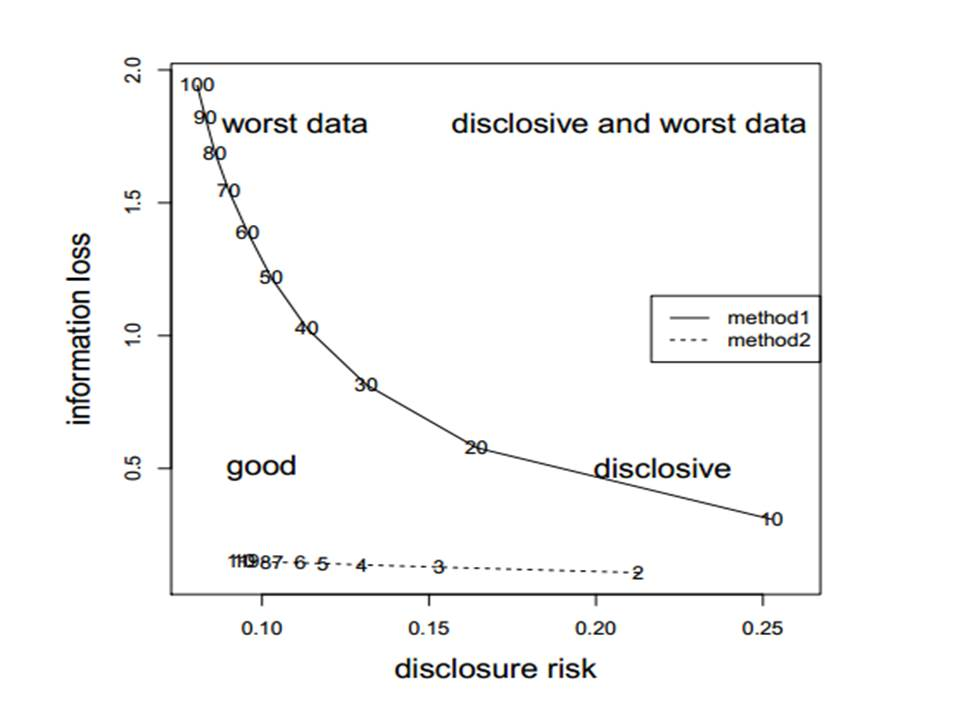
\includegraphics[width=0.99\linewidth]{JPEGS/TemplGraph1}
\end{figure}

\end{frame}
%============================================== %
\begin{frame}
		\frametitle{Risk Versus Data Utility}
\begin{itemize}
\item For Method 1 (in this example adding noise), the parameter varies between 10
(small perturbation) to 100 (perturbation is 10 times higher). 
\item When the parameter
value is 100, the disclosure risk is low since the data are heavily perturbed, but the

information loss is very high, which also corresponds to very low data utility. 
\end{itemize}

%--------------------------Page 3 / 31
%% 1 CONCEPTS
\end{frame}
%============================================== %
\begin{frame}
	\frametitle{Risk Versus Data Utility}
\begin{itemize}
\item When
only low perturbation is applied to a dataset, both risk and data utility are high. 
\item It
is easy to see that data anonymized with Method 2 (we used microaggregation with
different aggregation levels) have considerably lower risk; therefore, this method
is preferable.
\end{itemize}
\end{frame}
%============================================== %
\begin{frame}
		\frametitle{Risk Versus Data Utility}
\begin{itemize}
\item In addition, information loss increases only slightly if the parameter
value increases; therefore, Method 2 with parameter value of approximately 7
would be a good choice in this case since this provides both, low disclosure risk
and low information loss. 
\end{itemize}
\end{frame}
%============================================== %
\begin{frame}
	\frametitle{Risk Versus Data Utility}
	\begin{itemize}
\item For higher values, the perturbation is higher but the
gain is only minimal, lower values reports higher disclosure risk, Method 1 should
not be chosen since the disclosure risk and the information loss is higher than for
method 2. \item However, if for some reasons method 1 is chosen, the parameter for
perturbation might be chosen around 40 if 0.1 risk is already considered to be
safe. 
\item For data sets concerning very sensible information (like cancer) the might
be, however, to high risk and a perturbation value of 100 or above should then be
chosen for method 1 and a parameter value above 10 might be chosen for method
\end{itemize}
\end{frame}
%============================================== %
%\begin{frame}
%\begin{itemize}
%\item Figure 1: Risk versus information loss obtained for two specific perturbation meth-
%ods and different parameter choices applied to SES data o11 continuous
%scaled variables. Note that the information loss for the original data is
%O and the disclosure risk is 1 respecively, i.e. the two curves starts from
%(1,0).
%\end{itemize}
%\end{frame}
%============================================== %
\begin{frame}
\textbf{Considerations}
	\begin{itemize}
\item In real-world examples, things are often not as clear, so data anonymization specialists should base their decisions regarding risk and data utility on the following
considerations:
%Page 4 / 31
%
%
%
%1 CONCEPTS

\item What is the legal situation regarding data privacy? Laws on data privacy vary
between countries; some have quite restrictive laws, some don’t, and laws often
differ for different kinds of data (e.g., business statistics, labor force statistics,
social statistics, and medical data).

\end{itemize}
\end{frame}
%============================================== %
\begin{frame}
	\begin{itemize}

\item How sensitive is the data information and who has access to the anonymized
data file? Usually, laws consider two kinds of data users: users from universities
and other research organizations, and general users, i.e., the public. In the first
case, special contracts are often made between data users and data producers.

\item Usually these contracts restrict the usage of the data to very specific purposes, and
allow data saving only within safe work environments. For these users, anonymized
microdata files are called scientific use files, whereas data for the public are called
public use files. Of course, the disclosure risk of a public use ile needs to be very
low, much lower than the corresponding risks in scientific use files. For scientific
use files, data utility is typically considerably higher than data utility of public use
files.

\end{itemize}
\end{frame}
%============================================== %
\begin{frame}
	\begin{itemize}
\item Another aspect that must be considered is the sensitivity of the dataset. Data
011 individuals’ medical treatments are more sensitive than an establishment’s
turnover values and number of employees. If the data contains very sensitive in-
formation, the microdata should have greater security than data that only contain
information that is not likely to be attacked by intruders.
\end{itemize}
\end{frame}
%============================================== %
\begin{frame}
	\begin{itemize}
\item Which method is suitable for which purpose? Methods for Statistical Disclosure Control always imply to remove or to modify selected variables.
\item \textbf{Key} The data
utility is reduced in exchange of more protection. 
\item While the application of some
specific methods results in low disclosure risk and large information loss, other
methods may provide data with acceptable, low disclosure risks. 

\end{itemize}
\end{frame}
%============================================== %
\begin{frame}
\textbf{Recommendations (or lack thereof)}
	\begin{itemize}
\item General recomendations can not be given here since the strenghtness and weakness of methods
depends on the underlying data set used.
\item  Decisions on which variables will be
modified and which method is to be used result are partly arbitrary and partly
result from a prior knowledge of what the users will do with the data.
\end{itemize}
\end{frame}
%============================================== %
\begin{frame}
	\begin{itemize}
\item Generally, when having only few categorical key variables in the data set, recoding and local suppression to achieve low disclosure risk for categorical key
variables is recommended. 
\item In addition, in case of continous scaled key variables,
microaggregation is easy to apply and to understand and gives good results.
\item  For
more experienced users, shuffling may often give the best results as long a strong
relationship between the key variables to other variables in the data set is present.

\end{itemize}
\end{frame}
%============================================== %
\begin{frame}
\begin{itemize}
\item In case of many categorical key variables, post—randomization might be applied
to several of these variables. Still methods, such as post—randomization (PRAM),
may provide high or low disclosure risks and data utility, depending on the specific
choice of parameter values, e.g. the swapping rate.
\end{itemize}
\end{frame}
%============================================== %
\begin{frame}
\begin{itemize}
		\item Beside these recommendations, in any case, data holders should always estimate
the disclosure risk for their original datasets as well as the disclosure risks and
data utility for anonyrnized versions of the data. 
\item To achieve good results (i.e., low
disclosure risk, high data utility), it is necessary to anonyrnize in an explanatory
manner by applying different methods using different parameter settings until a
suitable trade-off between risk and data utility has been achieved.
\end{itemize}
\end{frame}
\end{document}